\clearpage

\section{Different performance metrics}\label{apx:metrics-review}
There are many different ways of evaluating the pipeline performance found in the field of pose estimation. Some of the evaluations include the following:
\mdeff{Shall we keep this? Not as a bullet list for sure.} \lau{Maybe in the Appendix, but not in the main text imo.}
\begin{itemize}
\item Intersection over Union (IoU) of the object 3D cloud with a custom threshold classifying it as a good estimate or not (e.g. in the paper~\cite{10.1007/s11263-014-0733-5} the threshold score above 0.5 is considered good estimation).
\item Translation and rotation error between estimated 3D model and true 3D model with fixed thresholds (e.g. in the paper~\cite{shotton2013scene} they require the translation error to be below 5 cm and rotation error to be below 5\degree)
\item The average distance of all the points of the model from their transformed version, and if the error is less than the constant multiple of diameter of the 3D model, it is considered correctly evaluated (e.g. evaluation error is used in papers \cite{10.1007/978-3-642-37331-2_42, xiang2018posecnn})
\item Reprojection error that projects the estimated points onto the image and computes the pairwise distances in the image space, instead of computing distances in the 3D model space (e.g. used in paper~\cite{xiang2018posecnn})
\item The recovery error measured as Frobenius norm from estimated 3D model and true model, where 3D model is composed of 3D locations of important landmarks (e.g. elbow for human pose estimation)~\cite{wangni2018monocular}
\item Average Orientation Similarity (AOS) is the difference between the true and estimated model with a cosine similarity term~\cite{RedondoCabrera2016PoseEE}
\item Mean Angle Error (MAE) and Median Angle Error (MedError) evaluated and compared with other pose estimation error metrics in the paper~\cite{RedondoCabrera2016PoseEE}.
\end{itemize}

\section{Orientation recovery: Recovery from exact distances}\label{apx:results:orientation-recovery:exact}

%\mdeff{Story: works perfectly despite no convexity guarantee and sampling.}
%\mdeff{I made it concise but precise. Let's do that for all!}

To verify that (i) the lack of a convexity guarantee for \eqnref{orientation-recovery} and (ii) the severe sampling of the sum are non-issues in practice, we attempt orientation recovery under exact distance estimation $d_p(\p_i, \p_j) = d_q(q_i, q_j)$.
%\mdeff{With $7000$ steps we actually don't under-sample, as $7000 \times 256 > P^2-P)/2 \approx \num{350e3}$.}
From $P_{\text{test}}=838$ projections taken from the asymmetric protein \texttt{5j0n}, we randomly sample batches of $256$ pairs (out of $(P^2-P)/2 \approx \num{350e3}$) at every step and minimize \eqnref{orientation-recovery} with the Adam optimizer~\cite{kingma2014adam} for $\num{7000}$ steps ($\sim 1.4$ hour) with a learning rate of $0.5$.
Orientations are perfectly recovered.
\figref{5j0n-orientation-recovery-loss} shows the convergence of~\eqnref{orientation-recovery} to zero.

\begin{figure}[ht!]
    \centering
    %\begin{subfigure}[b]{0.45\textwidth}
        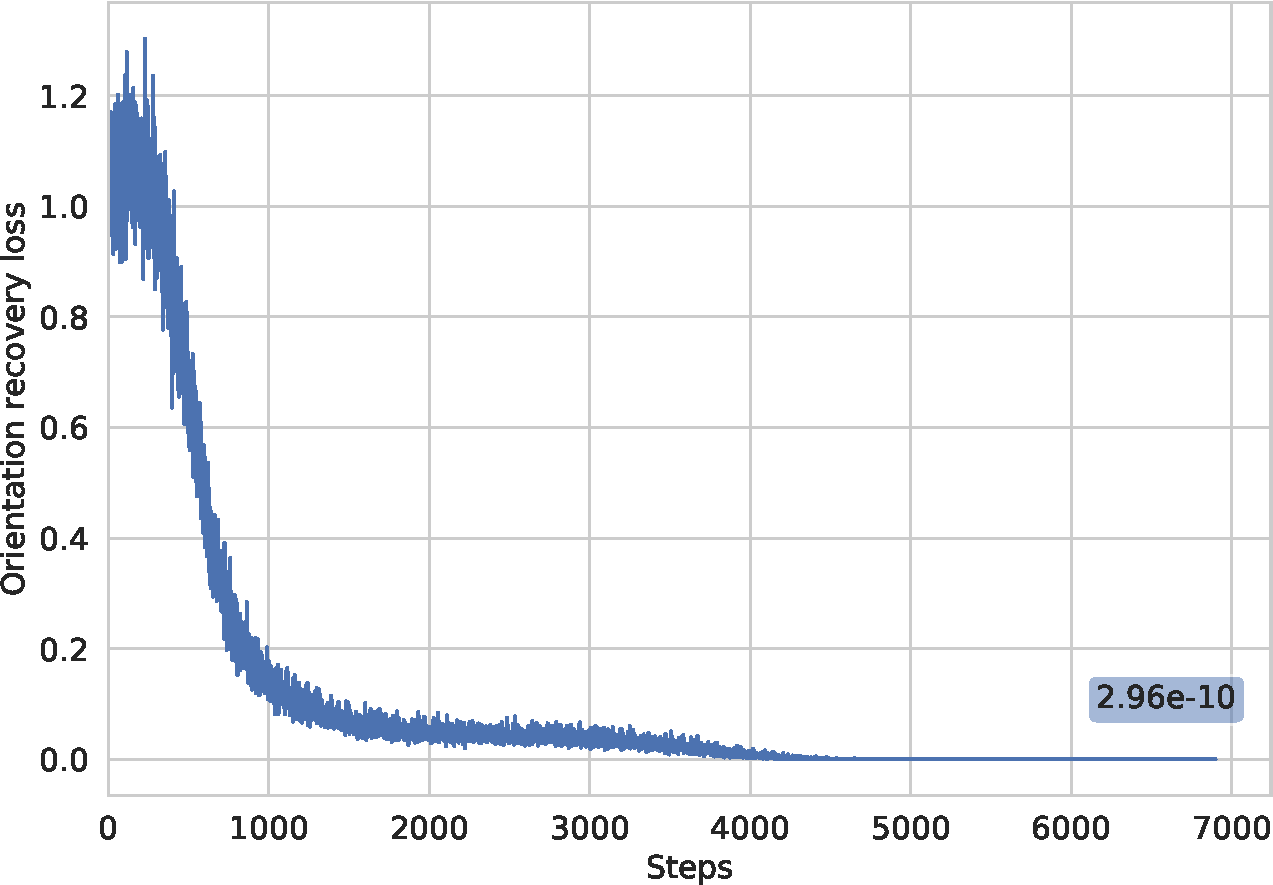
\includegraphics[height=7cm]{figures/5j0n_perfect_angle_recovery}
        %\caption{Asymmetric protein (\texttt{5j0n}).}
    %\end{subfigure}
    %\hfill
    %\begin{subfigure}[b]{0.5\textwidth}
    %\centering
    %    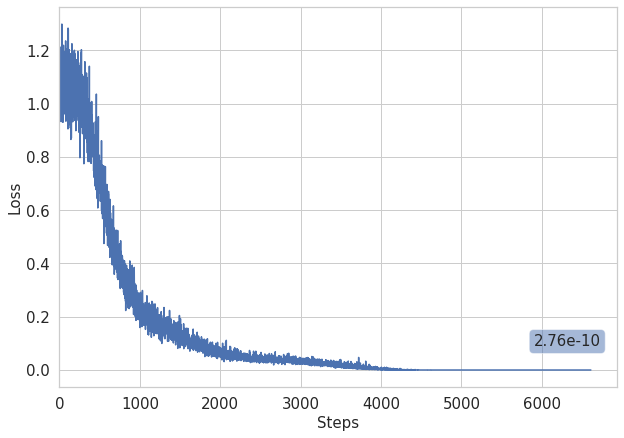
\includegraphics[height=5.5cm]{figures/5a1a_perfect_angle_recovery}
    %    \caption{Symmetric protein (\texttt{5a1a}).}
    %\end{subfigure}
    \caption{
        Example of perfect orientation recovery (for \texttt{5j0n}).
        The loss~\eqnref{orientation-recovery} converges to zero when the distance estimation is perfect, i.e., $d_p(\p_i, \p_j) = d_q(q_i, q_j)$.
    }\label{fig:5j0n-orientation-recovery-loss}
\end{figure}

Empirically we find that the mean orientation recovery error \eqnref{orientation-recovery-error} $E = 0$.
The sphere coverage before and after the orientation alignment can be seen in the \figref{5j0n-aa-loss-perfect-distances}.
We can see that the orientation alignment was performed successfully.

\begin{figure}[ht!]
    \centering
    \begin{subfigure}[b]{0.45\textwidth}
        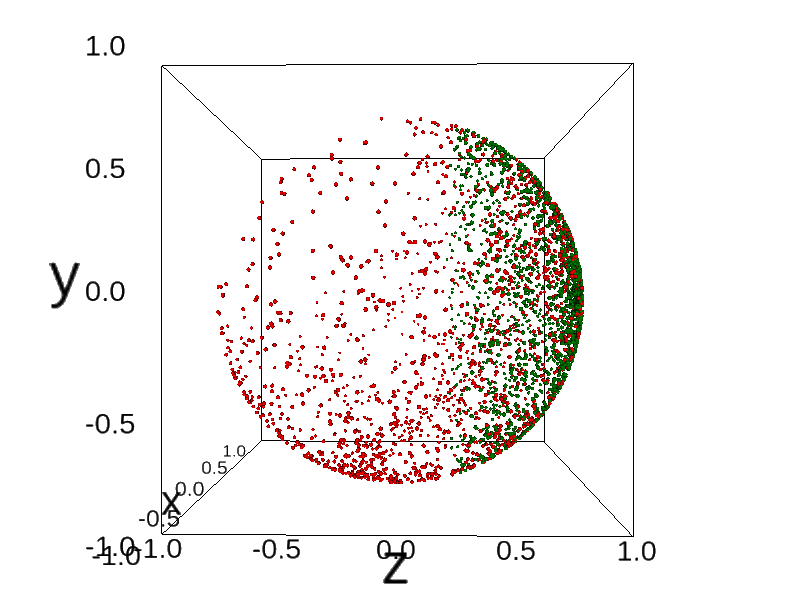
\includegraphics[height=6cm]{figures/coverage_alignment_before}
        \caption{Orientations before alignment.}
    \end{subfigure}
    \hfill
    \begin{subfigure}[b]{0.50\textwidth}
    \centering
        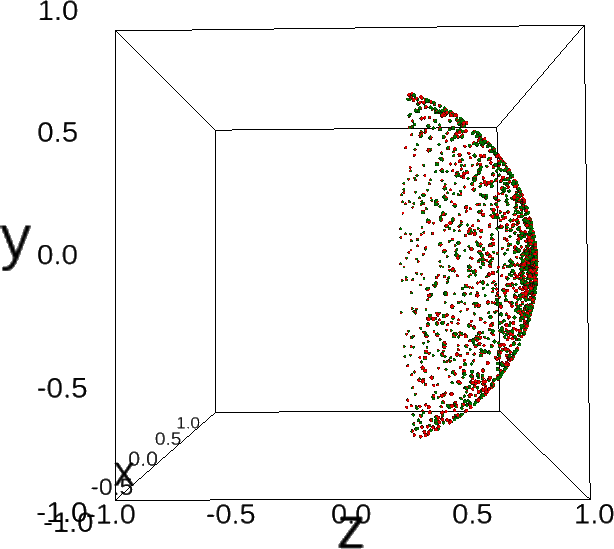
\includegraphics[height=6cm]{figures/coverage_alignment_after}
        \caption{Orientations after alignment.}
    \end{subfigure}
    \\
    \begin{subfigure}[b]{0.45\textwidth}
        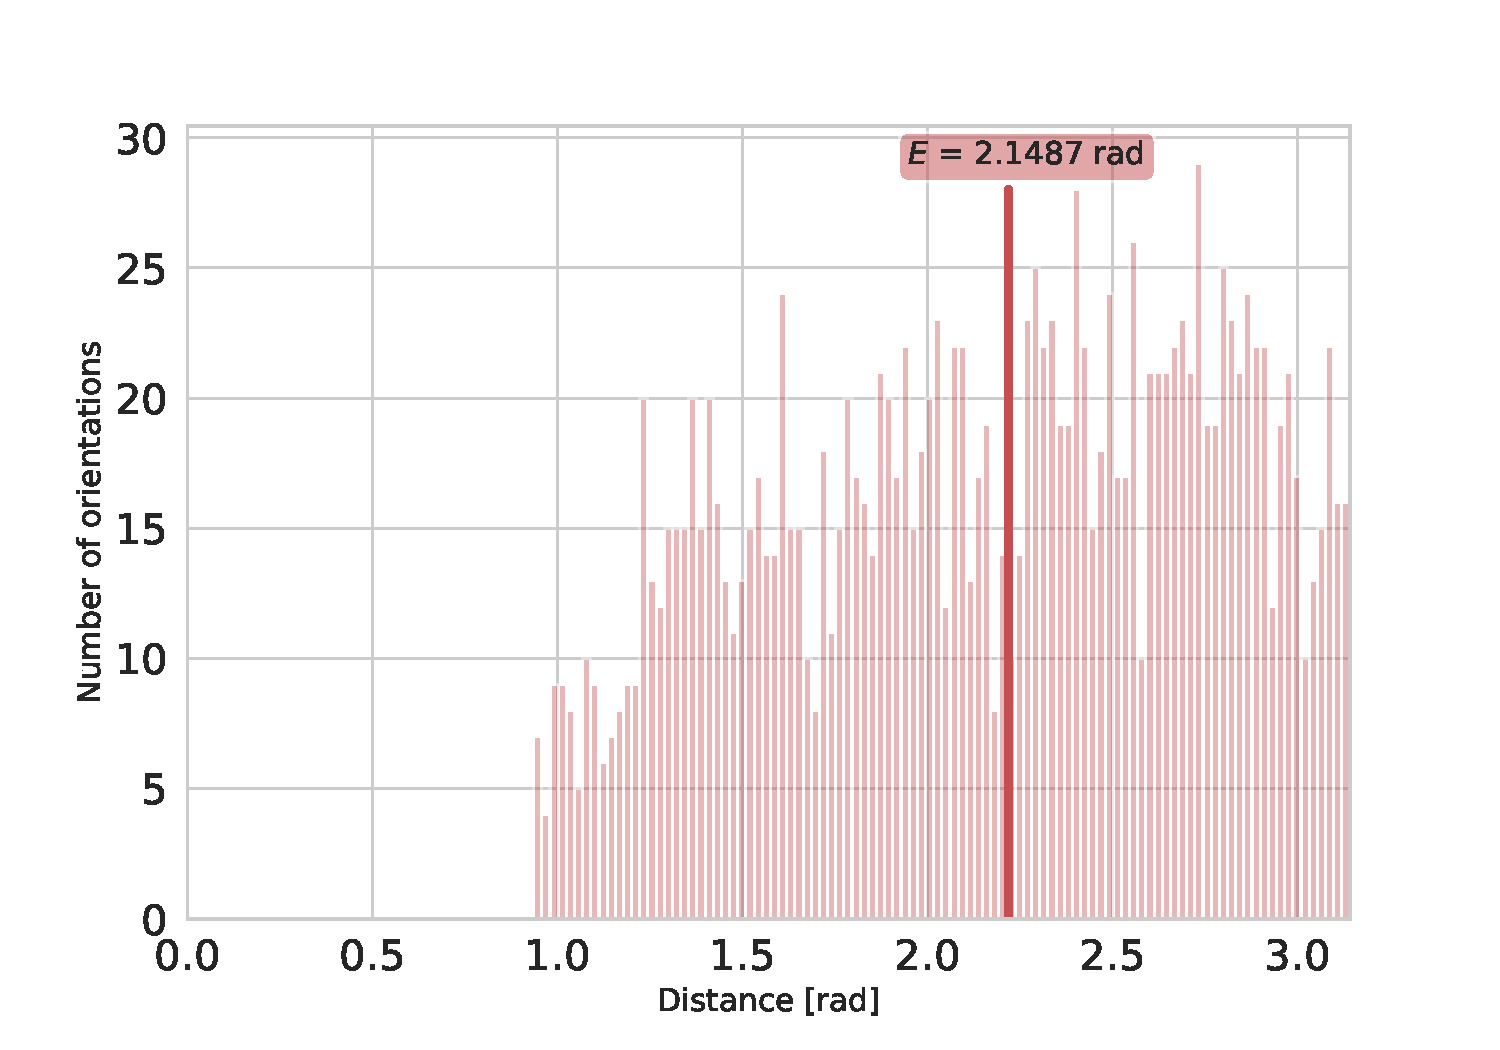
\includegraphics[height=5.5cm]{figures/5j0n_perfect_angle_ralignment_before}
        \caption{Orientation recovery error without alignment.}
    \end{subfigure}
    \hfill
    \begin{subfigure}[b]{0.5\textwidth}
    \centering
        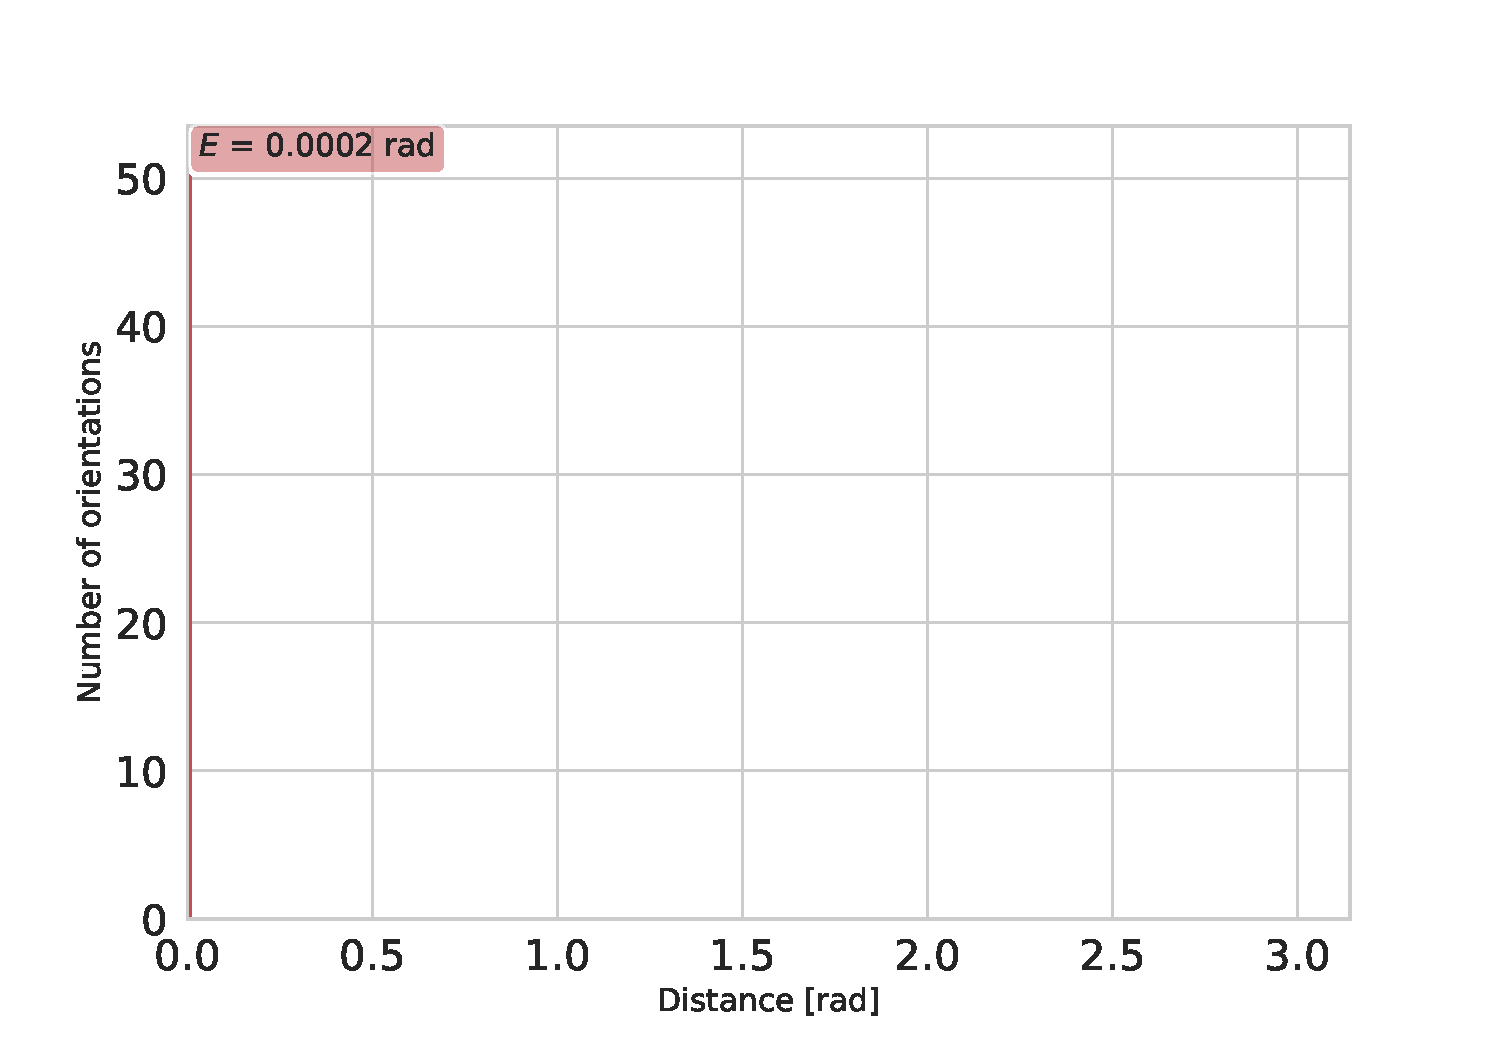
\includegraphics[height=5.5cm]{figures/5j0n_perfect_angle_ralignment_after}
        \caption{Orientation recovery error with alignment.}
    \end{subfigure}
    \caption{%
        Example of perfect alignment after a perfect orientation recovery under the true distance $d_p(\p_i, \p_j) = d_q(q_i, q_j)$ (\texttt{5j0n}).
        The first row shows the orientation coverage of $\mathbb{S}^2 \subset \SO(3)$ after the recovery.
        Green points are the ground truth orientations ${\{q_p\}}_{p=1}^P$ and red points are the recovered orientations ${\{\widehat{q_p}\}}_{p=1}^P$. The Figure (b) is exactly aligned which can be seen when zoomed. Due to plotting artifacts, both colors can still be seen.
        % orientations projected on S²
        The second row are the histograms of ${\{ d_q (q_p, \T \widehat{q_p}) \}}_{p=1}^P$, with $\T = \mathbf{I}$ on the left (i.e., without alignment) and $\T$ as the optimum of \eqnref{orientation-recovery-error} on the right.
        Alignment is necessary to evaluate the performance of orientation recovery.
    }\label{fig:5j0n-aa-loss-perfect-distances}
%    \label{fig:angle-alignment-perfect}
\end{figure}

\section{Distance estimation: Euclidean distance}\label{apx:results:distance-estimation}
%\subsection{Estimating Relative Orientations from Projections}
%\subsection{Relative orientation estimation}

%\mdeff{Story: $d_p$ good estimator of $d_q$.
%SiameseNN better than l2, but still plateaus.
%Robust to projection noise.}

The challenge of distance estimation is to define the distance between two projections $d_p$ such that it is connected to the distance between two quaternions $d_q$. We start by using the Euclidean distance as the baseline. Then, we learn the distance metric using the SiameseNN architecture. With this network we aim to classify the new unseen pairs of projections without training the network again. Afterwards, we explore different network architectures as well as test the sensitivity of the network to perturbed projections.

%\subsubsection{Euclidean distance}\label{sec:results:distance-estimation:euclidean}

%\mdeff{Story: simplest baseline estimator, $d_{pe}$ somewhat estimates $d_q$, quickly plateaus (even in the simplest noiseless and centered case).
%Note the difference between symmetric and asymmetric proteins.}

We evaluate $d_p(\p_i, \p_j) = \Vert \p_i - \p_j \Vert_2$ (i.e., the Euclidean distance) as a baseline distance estimator.
From $P = 5,000$ possible projection, we randomly select $5$ projections.
For each of these projections, we compute the Euclidean distance between aforementioned projection and all the others $d_p(\mathbf{p}_i,\mathbf{p}_j)=\lVert\mathbf{p}_i-\mathbf{p}_j\rVert_2$ and their corresponding orientation distance $d_q(q_i,q_j)$ through~\eqnref{distance:orientations}.
We then report the $(d_q,d_p)$ relationship for all pairs in \figref{euclidean-not-robust}, for both the asymmetric protein (left) and the symmetric one (right).

\begin{figure}[ht!]
    \centering
    \begin{subfigure}[t]{0.45\textwidth}
        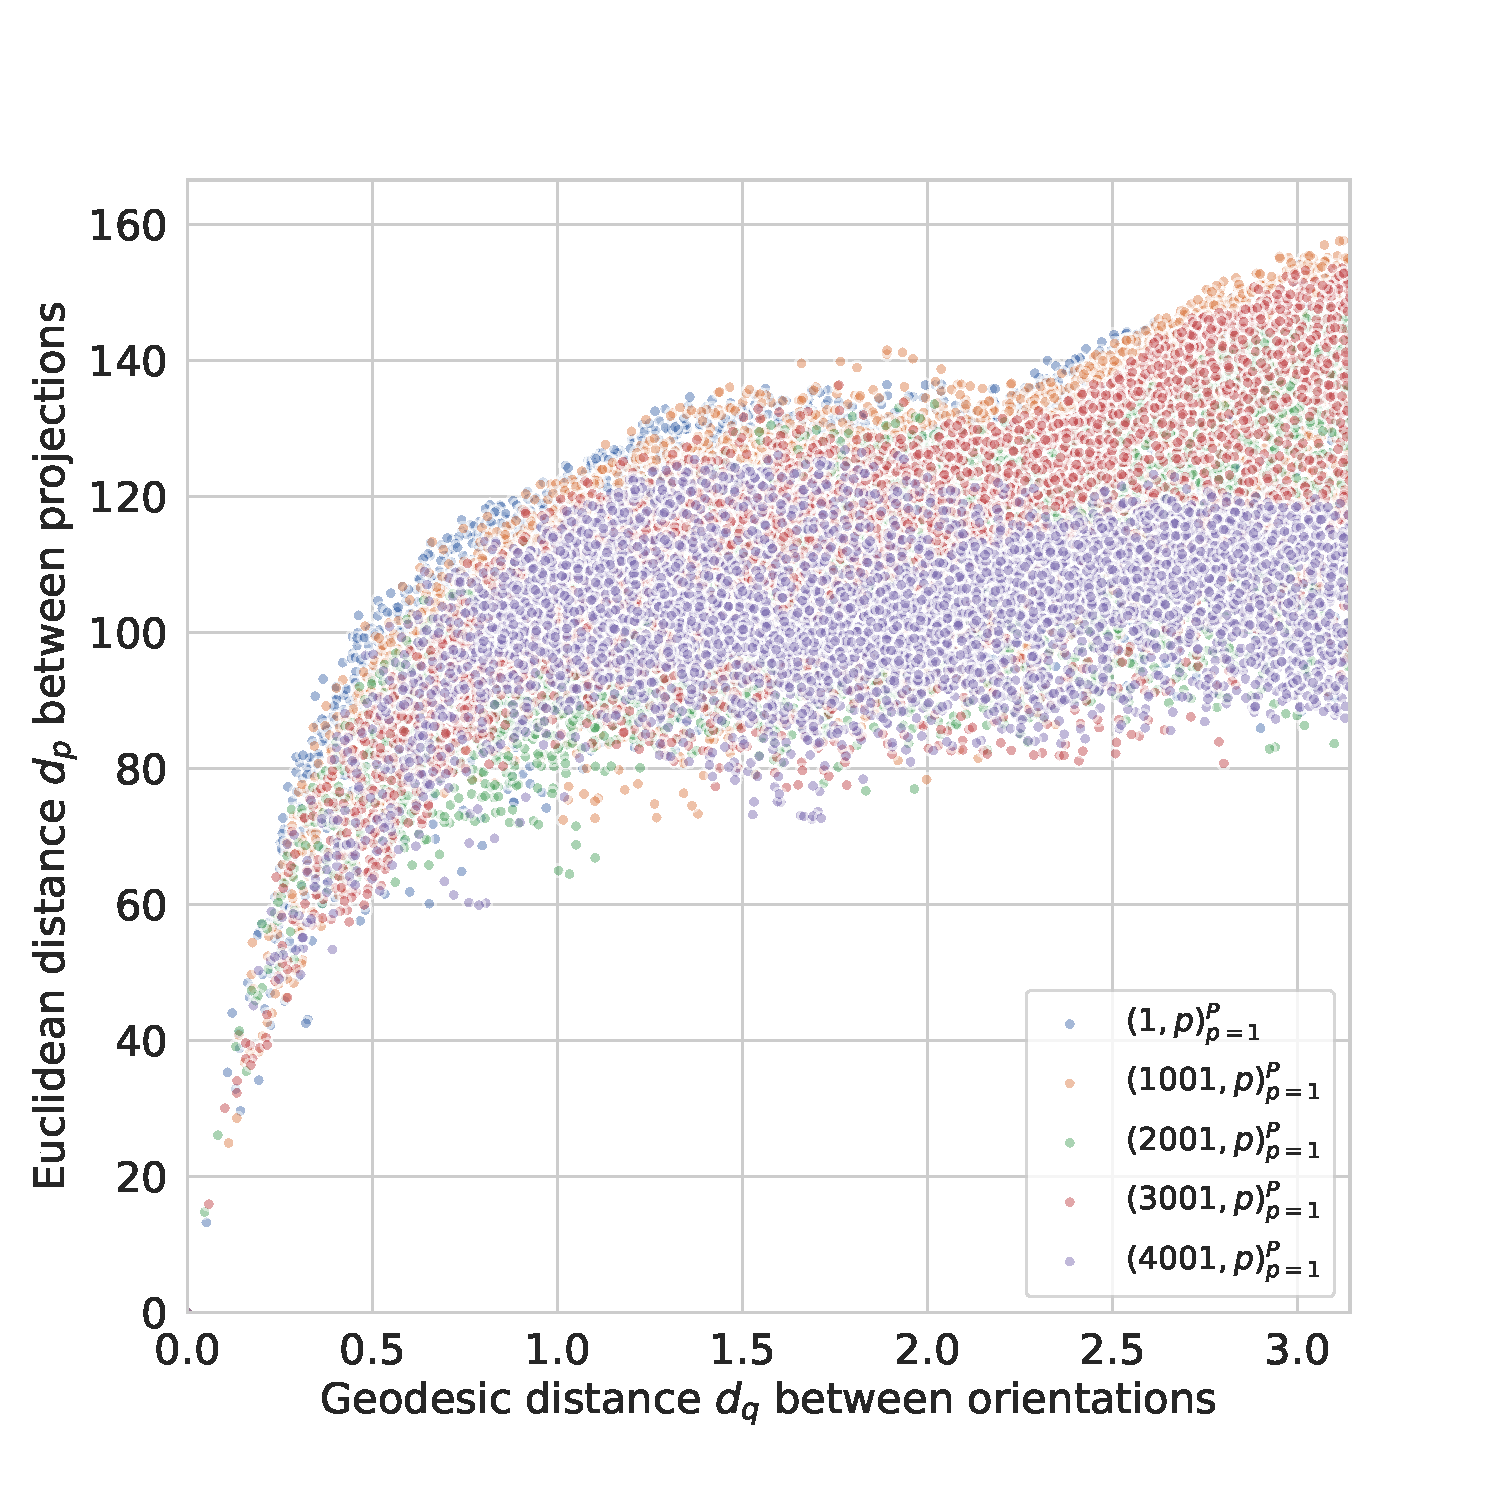
\includegraphics[height=7.5cm]{figures/eucl_notrobust_5j0n}
        \caption{Asymmetric protein (\texttt{5j0n}).}
    \end{subfigure} \quad \quad
    \begin{subfigure}[t]{0.45\textwidth}
        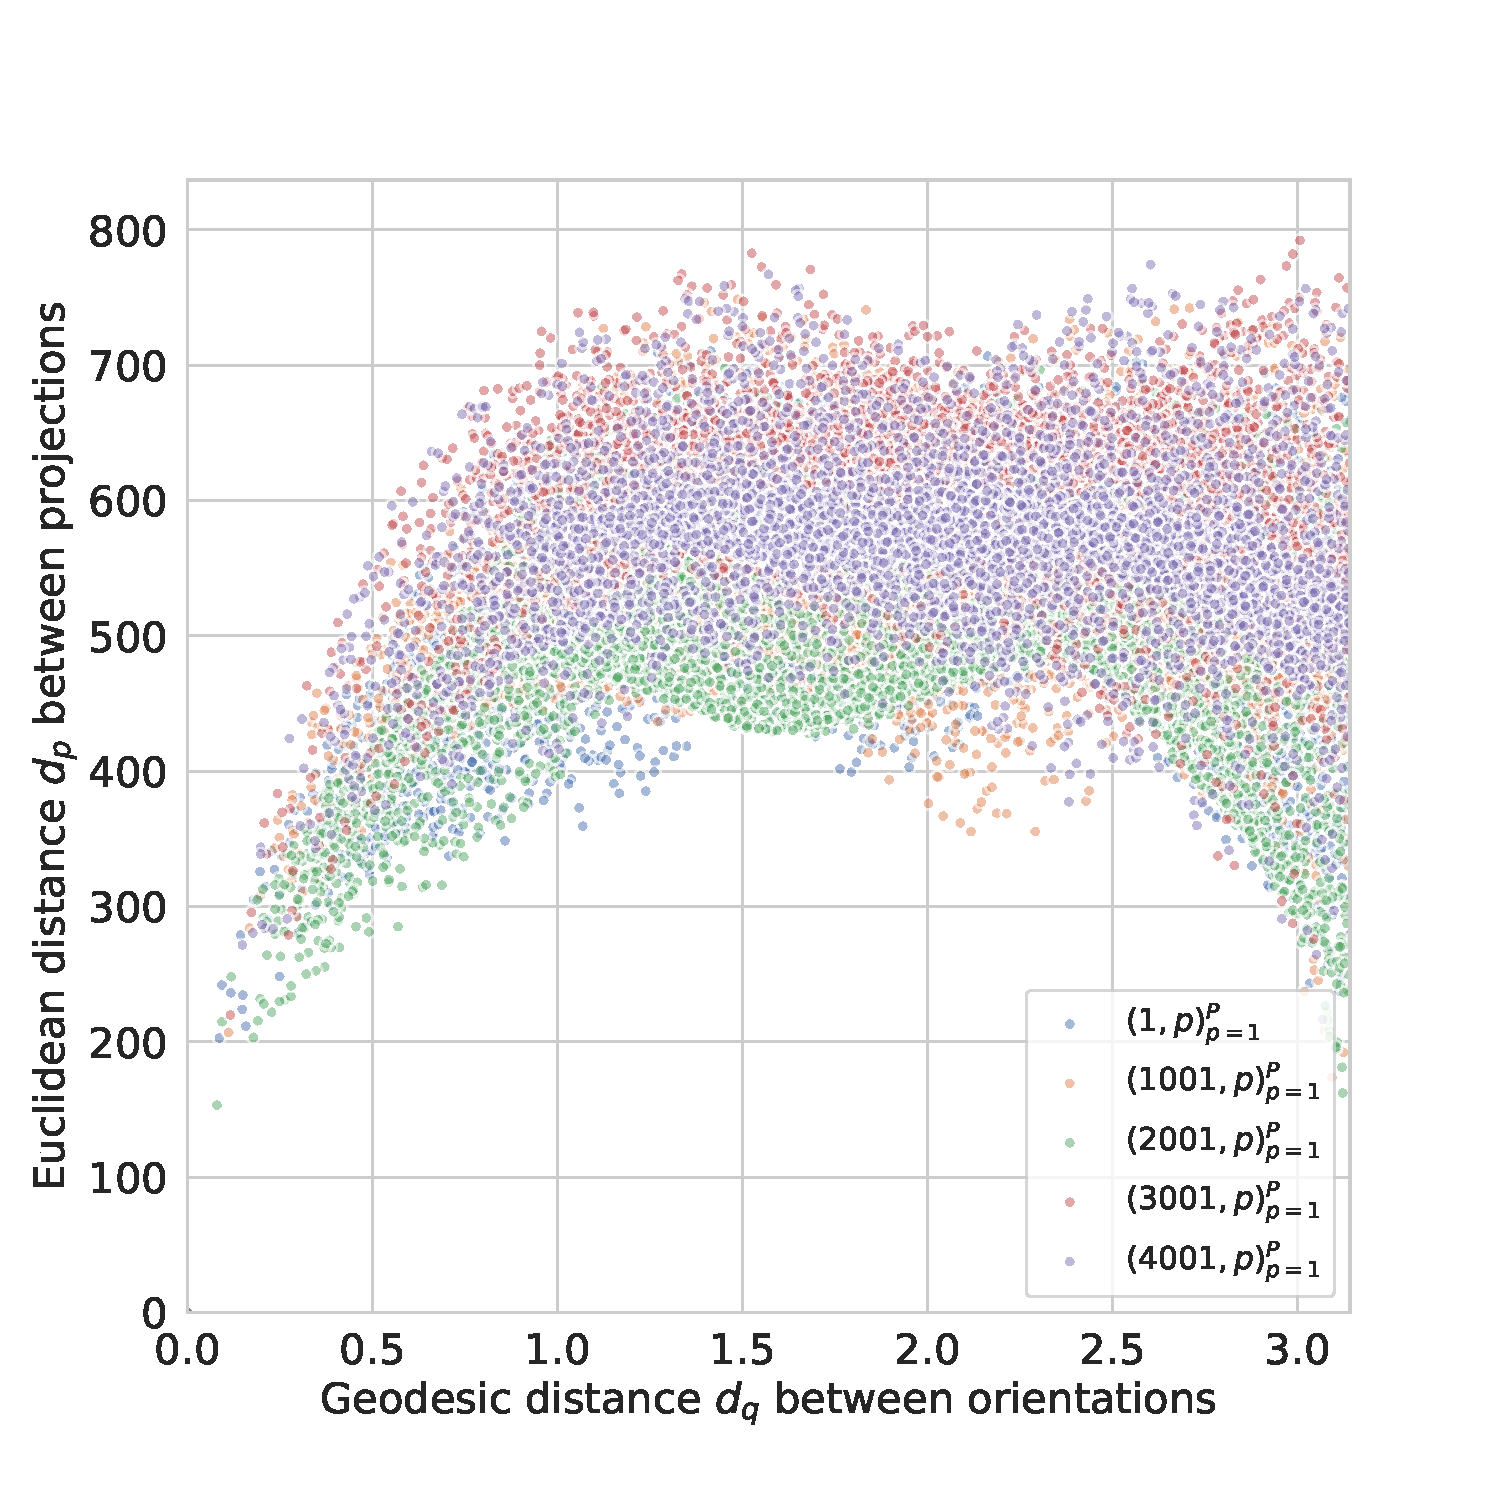
\includegraphics[height=7.5cm]{figures/eucl_notrobust_5a1a}
        \caption{Symmetric protein (\texttt{5a1a}).}
    \end{subfigure}
    \caption{
        Plotting the Euclidean distance between two projections versus their actual relative orientation (measured by the geodesic distance) for \textbf{(left)} the asymmetric protein (\texttt{5j0n}) dataset, and \textbf{(right)} the symmetric protein (\texttt{5a1a}) dataset.
        The color corresponds to projection pairs that share the first projection \textit{i.e.} distance between one projection with all other projections.
        %\todo{Figure label: ${\{(0, p)\}}_{p=1}^P$?}
    }\label{fig:euclidean-not-robust}
\end{figure}

Two principal observations can be made from this experiment.
First, as suspected, $d_p$ fails to be a consistent predictor of $d_q$, even in the simple imaging conditions considered here (no noise, no translation, no PSF).
In particular, the larger the quaternion distance $d_q$, the poorer the predictive ability of $d_p$ (the plot plateaus).
The other interesting observation is that the trend of $(d_q,d_p)$ plot of the $\beta$-galactosidase protein (\texttt{5a1a}) appears to take symmetric shape of letter \texttt{M} which can be explained with the fact that this protein has intrinsic dihedral (D2) symmetry~\cite{noauthor_d2sym_nodate,noauthor_5a1asym_nodate}.
%\mdeff{How does it appear?}

\section{Distance estimation: Influence of network architecture and feature distance}\label{apx:de-influence-arch}

%\mdeff{Story: $d_f = d_q$ better than Euclidean and MLP $d_f$. Architecture of $G_w$ doesn't seem to matter much. Surprising, because we don't overfit $\rightarrow$ future research needed.}

To further improve our network, we experiment with different feature distance metrics $d_f(\mathbf{f}_i,\mathbf{f}_j)$.
In the previous experiments we used the Euclidean distance as a features distance metric, \textit{i.e.} $d_f(\mathbf{f}_i,\mathbf{f}_j)=\lVert \mathbf{f}_i-\mathbf{f}_j\rVert_2$.
%\mdeff{Consistency: In \secref{method:distance-learning}, I used $d_f$  (for consistency with $d_p$ and $d_q$) and $\mathbf{f}_i$ (for consistency with $\p_i$ and $q_i$).}

In this experiment, we test the performance with a geodesic distance, \textit{i.e.}
\begin{equation*}
    d_f(\mathbf{f}_i,\mathbf{f}_j) = 2 \arccos \left( \frac{\mathbf{f}_i \cdot \mathbf{f}_j}{\lVert \mathbf{f}_i \rVert \lVert \mathbf{f}_j \rVert} \right) = 2 \arccos \left( \frac{\sum_{k=1}^n f_{i,k} f_{j,k}}{\sqrt{\sum_{k=1}^n f_{i,k}^2}\sqrt{\sum_{k=1}^n f_{j,k}^2 }} \right).
    \label{eqn:geodesic-distance}
\end{equation*}

Additionally, we parametrize $d_f(\mathbf{f}_i,\mathbf{f}_j)$ as MLP. It consists of six hidden linear layers with \texttt{1024}, \texttt{512}, \texttt{512}, \texttt{256}, \texttt{256}, and \texttt{1} unit respectively. All of them use SeLU as an activation function.

The experimental conditions are the same as in the previous section with the Euclidean distance metric as feature distance metric.
\figref{geo-eucl-mlp} shows the training and validation losses of the geodesic distance are better than Euclidean and MLP feature distance metric. We can also observe the performance on the $(d_q, d_p)$ plots and notice that the projection pairs deviate the least using the geodesic distance.
%\todo{Why? Add and rephrase hypotheses. Cosine distance has the same geometry as $d_q$. Euclidean has not (no periodicity nor curvature). MLP doesn't guarantee it's a distance function (not symmetric, zero between itself, triangle inequality) and might need much more data.}
The reason for a geodesic distance to perform the best is that it has the same geometry as quaternion distance $d_q$ in $\SO(3)$ space. Whereas, the Euclidean distance is not desirable on $\SO(3)$ since it does not respect the manifold's non-linearity (it has no periodicity nor curvature) and can lead to unpredictable behaviours. The $\SO(3)$ is non-linear and it can be explained with the fact that Euclidean distance of two quaternions can be small, despite the rotation being large~\cite{huynh_metrics_2009,DBLP:journals/corr/abs-1805-01026}.
Moreover, MLP does not guarantee that it is a distance function. For MLP to be a distance function, it should have the following properties: (1) support symmetry; (2) output zero with two identical inputs; (3) support triangle inequality. In addition, we might need much more data for the MLP training.
Hence, it is desirable to have a distance function that respects the structure of $\SO(3)$ space.

\begin{figure}
    \centering
    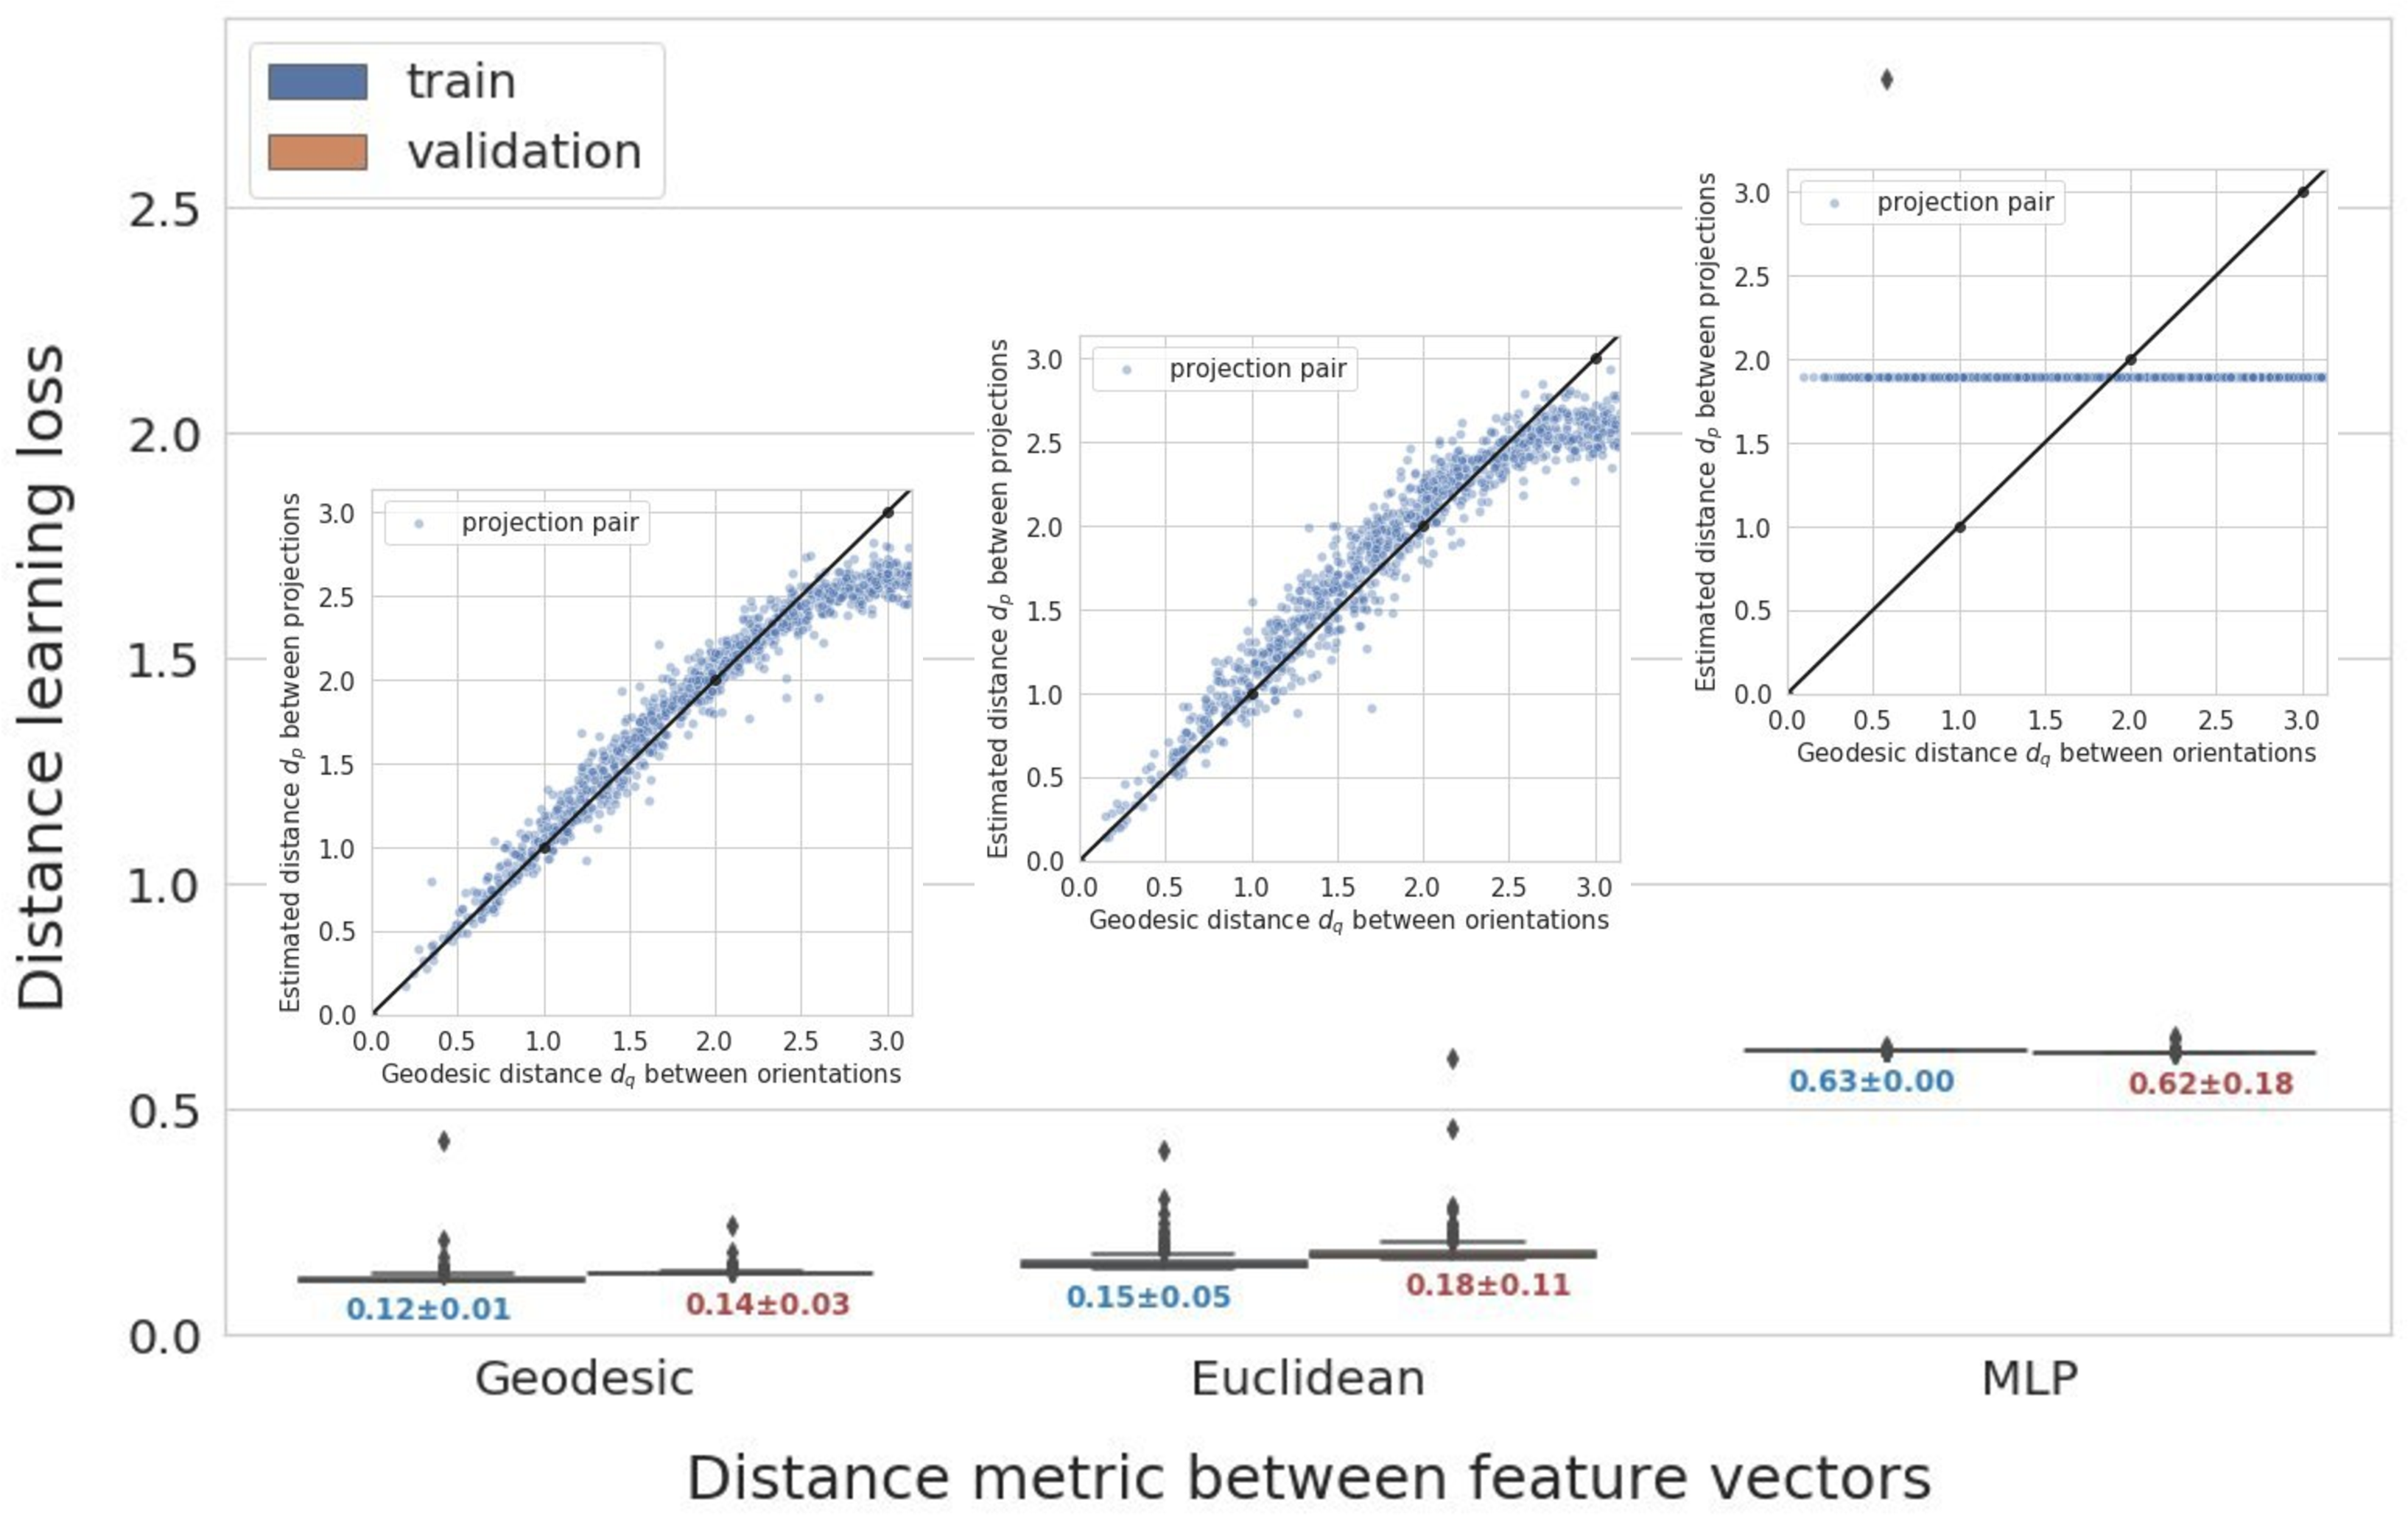
\includegraphics[height=7cm]{figures/geo_eucl_mlp_distance_metric.pdf}
    \caption{
        Training and validation epoch losses w.r.t. feature vectors' distance metric and their corresponding distance ratio $(d_q, d_p)$ plots.
    }\label{fig:geo-eucl-mlp}
\end{figure}

\clearpage
\section{SiameseNN architecture}\label{sec:siamese-architecture}

\begin{figure}[h!]
    \centering
    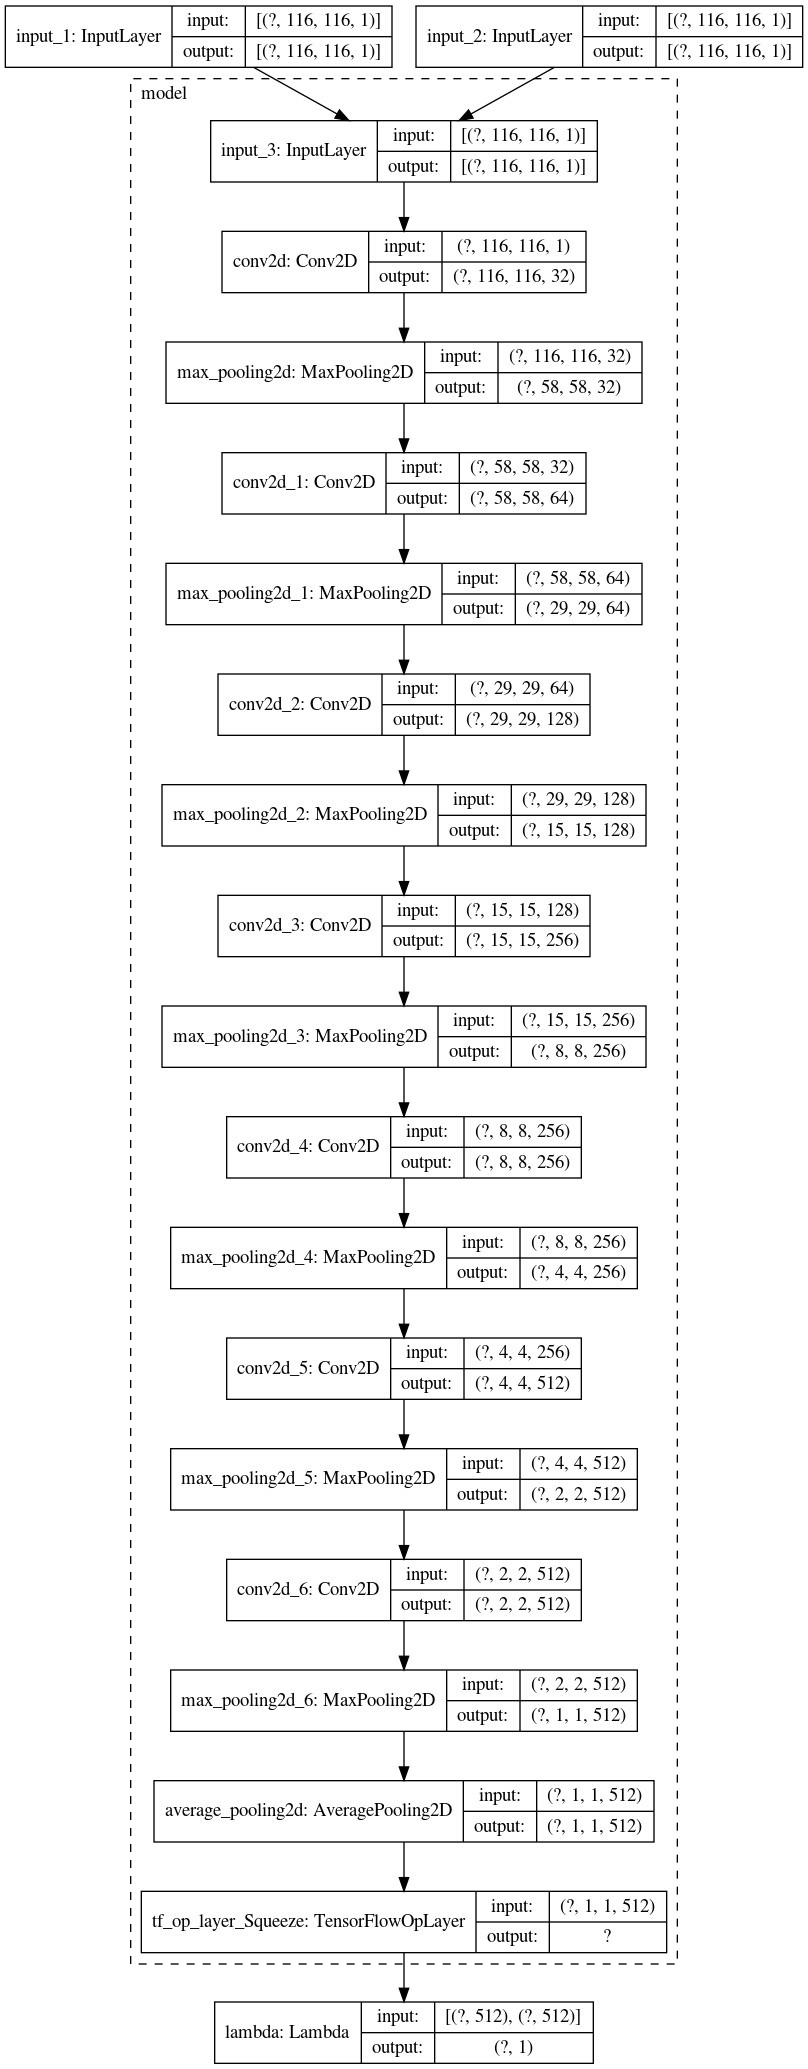
\includegraphics[height=19cm]{figures/model_plot.png}
    \caption{%
        Distance estimation network architecture.
        We have two input images of dimensions $116 \times 116$.
        Each one goes to its CNN (part where we share the weights).
        The output is a scalar value representing the distance between these two images.
    }\label{fig:de-architecture}
\end{figure}
